\documentclass{homework}
\usepackage{graphicx}
\author{Morales, Samantha}
\class{CSCI 2114: Tashfeen's Data Structures}
\date{\today}
\title{Homework 4}
\address{%
  Oklahoma City University, %
  Petree College of Arts \& Sciences, %
  Computer Science%
}

\acmfonts

\begin{document} \maketitle

You may download all the code for this homework at:
\url{https://tashfeen.org/s/ds/hw4code.zip}.

\question\label{plot} Recall from class the runtimes given in table \ref{runtime}.

\tbl<runtime>{Asymptotic runtime complexities for array lists and linked lists} {
  Data Structure\textbackslash Operation & Random Insert & Random Access \\
  Array List                             & $\O(n)$       & $\O(1)$       \\
  Linked List                            & $\O(1)$       & $\O(n)$       \\
}

In this question for each of the array list and linked list, we'll record times for
Java's,
\href{https://docs.oracle.com/javase/8/docs/api/java/util/List.html#add-E-}{List.add(E
  e)} and
\href{https://docs.oracle.com/javase/8/docs/api/java/util/List.html#get-int-}{List.get(int
  index)}. Note that both of the Java's \texttt{LinkedList} and
\texttt{ArrayList} implement the above \texttt{List} interface.

Finish implementing the Java class \texttt{ListExperiment}. Once
fully implemented, this class should give you two comma separated
files (CSV) with rows corresponding with nanoseconds taken to
append the $i^\text{th}$ element or perform a binary search in a
list of size $2^i$. Plot each row in these CSV files against their
index using your favourite plotting utility. You may use this
\texttt{plot\_list.py} (make sure you set the appropriate
variables) if you want. Give the two plots.

Do the plots confirm or overrule what we know about the runtimes
linked and array lists? Discuss.

\begin{sol}
  The search confirmed that linked list searches run in linear time and array list runs in constant time.
  The append confirmed that both append in constant time for the best case, however array list runs in linear for its worst case,
  while linked list continues to run in constant.
\end{sol}

\begin{figure}[htbp] % Adjust placement options as needed (h, t, b, p)
  \begin{minipage}[t]{0.45\textwidth} % Adjust width as needed, [t] aligns tops
    \centering
    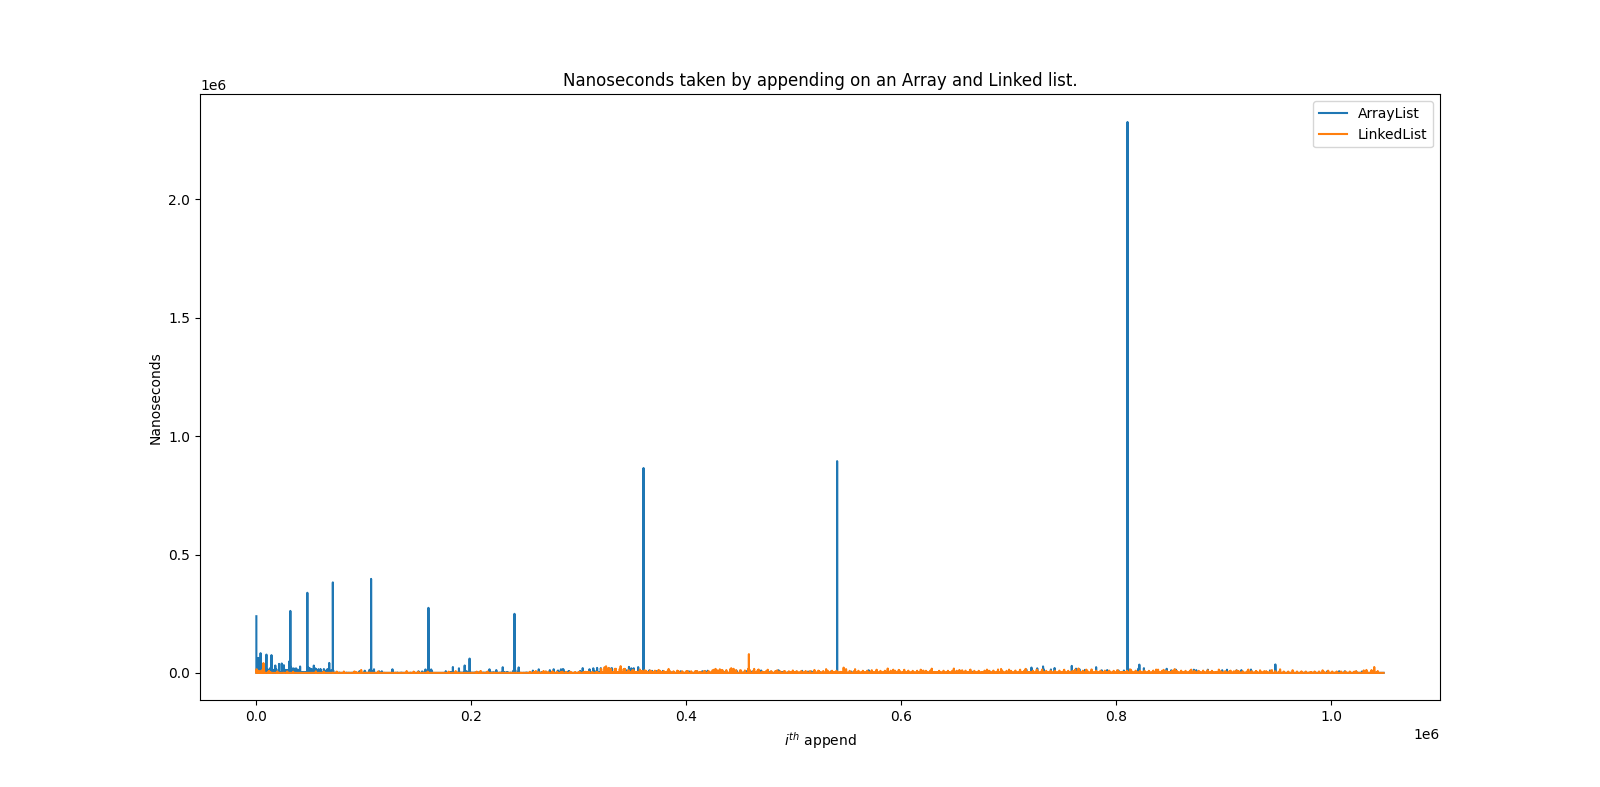
\includegraphics[width=\linewidth]{./media/List_append.png} % image1.png is your first image file
  \end{minipage}
  \hfil
  \begin{minipage}[t]{0.45\textwidth} % Adjust width as needed, [t] aligns tops
    \centering
    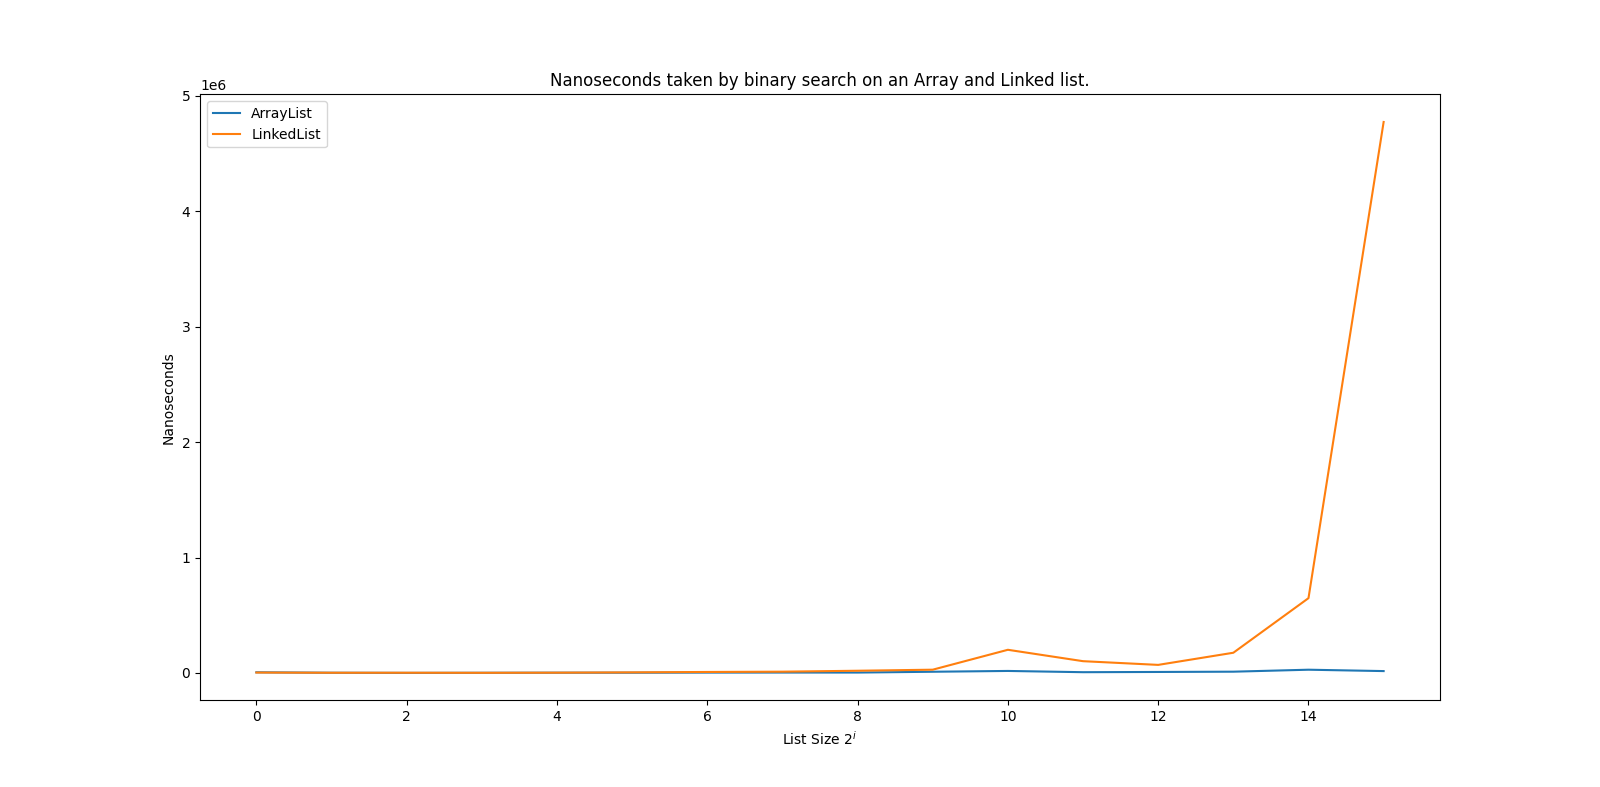
\includegraphics[width=\linewidth]{./media/List_search.png} % image1.png is your first image file
  \end{minipage}
  \caption{List Plots}
\end{figure}

\question Extend \texttt{Structure.java} to implement \texttt{Stack.java}
and \texttt{Queue.java} \ie
\begin{verbatim}
public class Queue<T extends Comparable<T>> extends Structure<T> {...}
\end{verbatim}
and
\begin{verbatim}
public class Stack<T extends Comparable<T>> extends Structure<T> {...}
\end{verbatim}

\begin{enumerate}
  \item Use your stack implementation to figure out that of 1,000,000
        randomly generated six character strings consisting of only `('
        and `)' \eg ``())())'' how many are balanced. I. e., ``())())'' is
        not balanced while ``()(())'' is balanced. State your answer as a
        ratio in the decimal point notation. Save the class in
        \texttt{Balance.java}.
  \item Use your queue implementation to draw the
        \href{https://en.wikipedia.org/wiki/Sierpi%C5%84ski_triangle}{Sierpinski's triangle}.
\end{enumerate}

\img<img3>[1]{Balanced.java Screenshot}{./media/BalancedScreenshot.png}
\img<img4>[0.65]{Sierpinski.java Screenshot}{./media/SierpinskiScreenshot.png}

\begin{lstlisting}[language=Java]
public class Sierpinski {
  public static void main(String[] args) {
    new Canvas(new Sierpinski());
  }
  public void points(int x, int y, int w, int h, Queue<Coordinates> q, int r) {
    // implement me.
  }
}
\end{lstlisting}

\question \sloppy Finish implementing the \texttt{BinaryHeap.java}. You need to implement the methods \\
\texttt{heapifyUp(Node<T> v)} and
\texttt{heapifyDown(Node<T> v)}. Run the file and verify your implementation keeps the heap property.

\img<img5>[0.65]{Binaryheap.java Screenshot}{./media/BinaryHeapScreenshot.png}

\section*{Submission Instructions}

\begin{enumerate}
  \item Turn in a PDF containing any plots, figures and/or answers from
        the homework.
  \item Turn in your, \texttt{ListExperiment.java, Stack.java, Queue.java, Balance.java, Sierpinski.java} and \texttt{BinaryHeap.java}.
\end{enumerate}

\end{document}
